%% ----------------------------------------------------------------
%% DataPreparation.tex
%% ---------------------------------------------------------------- 
\chapter{Data Preparation} \label{Chapter:DataPreparation}

\section{Dataset Explained}

The dataset was found and downloaded on the internet \cite{Dataset}, which is real data gathered in the city of Guiyang.
It contains both static and dynamic data throughout the years of 2015-2017, separated into three sets.

The first datasheet contains the information of a total of 132 links, the structure is shown in \fref{Figure:link_info}.
link\_ID is a string of unique IDs for each link; the length and width of the links are double values in meters; 
link\_class is the classification of the road, but since all the links in this data set are in class 1, this column has been eliminated for further processing.

\begin{figure}[!htb]
    \centering
    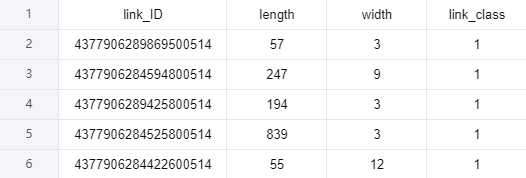
\includegraphics[width=10cm]{link info}
    \caption{First few samples of link info}
    \label{Figure:link_info}
\end{figure}

The second datasheet records the upstream and downstream relations of each link, forming the topology of the map. The structure is shown in \fref{Figure:link_top}.

\begin{figure}[!htb]
    \centering
    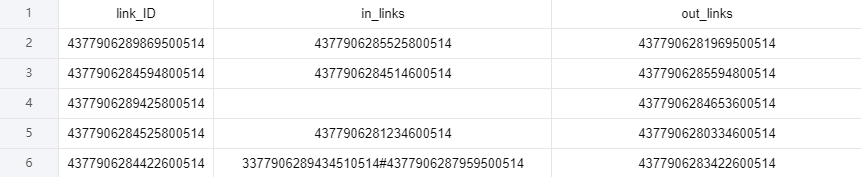
\includegraphics[width=14cm]{link top}
    \caption{First few samples of link topology}
    \label{Figure:link_top}
\end{figure}

The third datasheet is the records of the travel\_time (i.e. the average time of vehicles stays on the link) every two minutes (\fref{Figure:records}). 
A higher value of travel\_time means it takes a longer time for vehicles to pass the link, which implies the road is more congested. Hence, it is the value to predict. 
The datasheet also includes the record time interval and the date, including year and month, of the record. There are a total of 25,999,606 records, distributed mainly from March to June of 2016 and 2017.

\begin{figure}[!htb]
    \centering
    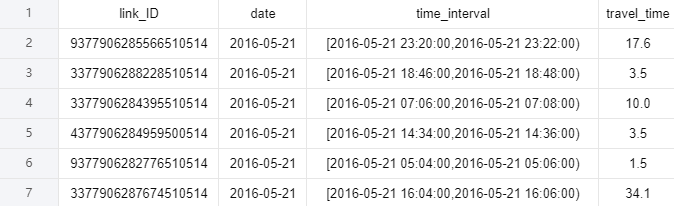
\includegraphics[width=12cm]{records}
    \caption{First few samples of records}
    \label{Figure:records}
\end{figure}

\section{Data Preparation and Evaluation}

Before the training of the model, the data needs to be analyzed first. For the RNN-based model, the data should be sorted in the sequence of time. 
With this implemented, the feature of time itself will not give much further characteristics, hence digging of the data to get more key features is vital before the training. 
This would potentially help to reach a better performance.

\subsection{Static Data}

\begin{figure}[!htb]
    \centering
    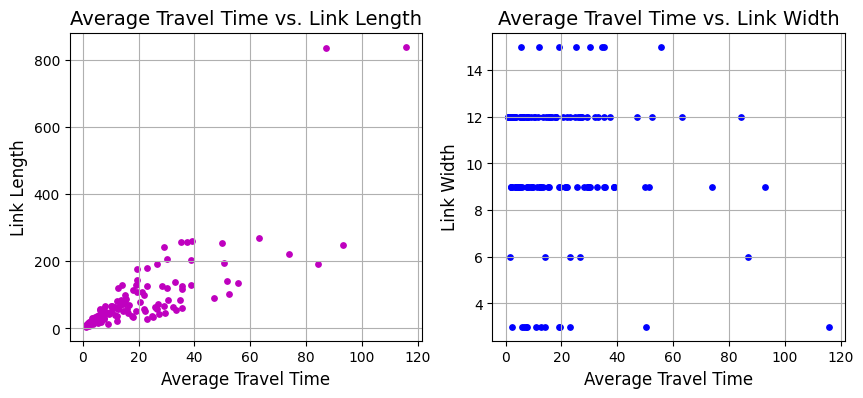
\includegraphics[width=12.5cm]{length_width_plot}
    \caption{Length \& Width vs. Average Travel Time}
    \label{Figure:length_width}
\end{figure}


The relation of the length and width of the links and the travel time has been studied, and the plot is shown in \fref{Figure:length_width}.
We can see that length has a strong positive correlation with travel time, whereas width seems not relevant at all. 

The upstream and downstream of links also are vital for prediction. It is planned to take them into account in the future. 

\subsection{Records}

The time indication features i.e. years, months, etc. are integer encoded. This might lead to the model incorrectly assuming magnitude relationships between categories. 
To eliminate this misunderstanding, one-hot encoding is used. The year contains only 2016 and 2017, which can be represented by 0 and 1, using one dimension of a sample.
The month includes every month from March to July, a total of 5 months, and five dimensions are occupied.

\begin{figure}[!htb]
    \centering
    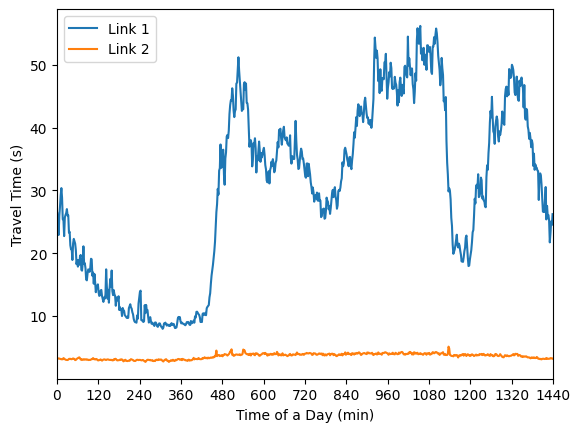
\includegraphics[width=8cm]{time of day}
    \caption{Time of day vs. average travel time of two randomly choosed links}
    \label{Figure:time_of_day}
\end{figure}

The time of the day also reveals characteristics for some of the links. \fref{Figure:time_of_day} shows the plot of two randomly chosen links.
Link1 varies a lot at different times. In contrast, Link2 gives a much flattened curve. Hour of day is decided to use as a feature, 
since it is also discrete, one-hot encoding is implemented. 

Whether it is a holiday also affects people's behaviour. Hence it would be reasonable to add a feature to tell if it is a holiday. 
Weekdays are also identified since some of the samples reveal periodicity throughout the week. 
By plotting them with the travel time on \fref{Figure:weekday_holiday}, it can be seen that the weekdays are generally higher in terms of travel time than holidays and weekends.

\begin{figure}[!htb]
    \centering
    \subcaptionbox{Holiday (1); Working day (0)}{
        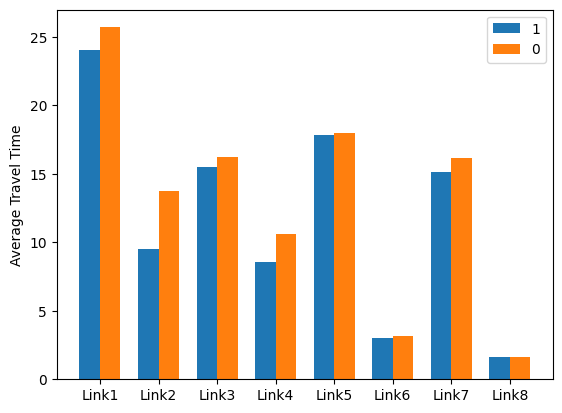
\includegraphics[width=7cm]{is holiday}
        \label{Figure:weekday_holiday:holiday}
    }
    \subcaptionbox{Weekend (1); Weekday (0)}{
        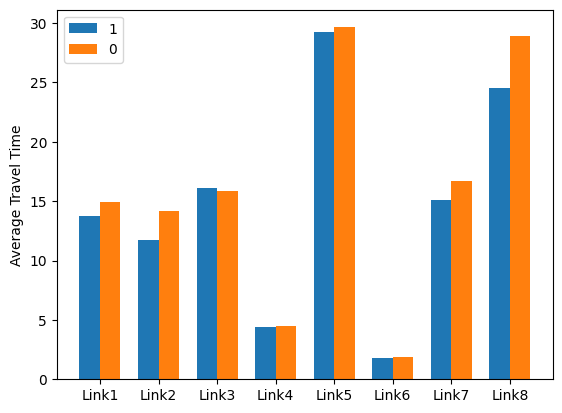
\includegraphics[width=7cm]{is weekend}
        \label{Figure:weekday_holiday:weekday}
    }
    \caption{8 randomly choosed links are used to compare (A) holiday (B) weekend with normal working day}
    \label{Figure:weekday_holiday}
\end{figure}

With everything above done, the data now have a dimension of 72 for each link. The structure is shown in \tref{Table:Dimensions}. 
There are 132 different links, each link is trained separately. 

\begin{table}[!htb]
    \centering
    \begin{tabular}{c|cc|c|cc}
    \toprule
    & length & type & & length & type \\
    \midrule
    year & 1 & bool & is\_holiday & 1 & bool \\
    month & 5 & bool & is\_weekend & 1 & bool \\
    weekday & 7 & bool & width & 1 & int \\
    day\_of\_month & 31 & bool & length & 1 & int \\
    hour\_of\_day & 24 & bool & speed & 1 & float \\
    time\_of\_day & 1 & int & travel\_time & 1 & float \\
    \bottomrule
    \end{tabular}
    \caption{Dimensions of samples for a single link}
    \label{Table:Dimensions}
\end{table}

It has been noticed that most links have missing data at various time segments.
Therefore, multiple methods were attempted to fill in the missing values. For the case where the missing values are sparse, i.e. two 
time segments before and after the sample are not missing, 
the average of the two segments before and after is used to fill in the gap. 
For large chunks of missing, drop the chunk in the training set, and fill the mean of the data of historical simultaneous moments in the test set. If fill the training set, it may cause large errors.
